% This file is iccc.tex.  It contains the formatting instructions for and acts as a template for submissions to ICCC.  It borrows liberally from the AAAI and IJCAI formats and instructions.  It uses the files iccc.sty, iccc.bst and iccc.bib, the first two of which also borrow liberally from the same sources. The format has been updated for the ICCC2022 to include a new, mandatory section to be included in camera-ready manuscripts.


\documentclass[letterpaper]{article}
\usepackage{iccc}


\usepackage{times}
\usepackage{helvet}
\usepackage{courier}
\usepackage{amsmath}
\usepackage{musicography}
\usepackage{graphicx}
\usepackage[font=small,skip=4pt]{caption}

\pdfinfo{
/Title (Formatting Instructions for Authors)
/Subject (Proceedings of ICCC)
/Author (ICCC)}
% The file iccc.sty is the style file for ICCC proceedings.
%
\title{Converting DNA to Music: Sonifying Splicing and Translation}
\author{Ilana Shapiro\\
Computer Science Department\\
Pomona College\\
Claremont, CA 91711 USA\\
issa2018@mymail.pomona.edu\\
}
\setcounter{secnumdepth}{0}

\begin{document} 
\maketitle
\begin{abstract}
The sonification of genetic material is a little-explored mode of unconventional computation that bridges the divide between bioinformatics, computer science, and music, allowing both scientists and the general public to perceptualize genomics in a novel and illuminating manner. This paper presents BioMus, an original model converting DNA to musical data as MIDI piano chords. Gene sequences are sourced from Ensembl, a genome database of the European Bioinformatics Institute, and are parsed into their constituent exons and and introns. Exons are further parsed into their 5' and 3' untranslated regions (UTRs) and CDS (CoDing Sequence, i.e. the spliced exons constituting the amino acid-coding sequence after UTRs are removed). Then, each codon in the CDS is mapped to a major or augmented triad based on the amino acid it codes for, and individual nucleobases in introns and UTRs are respectively mapped to diminished triads and dyads outlining a minor triad. Rhythmic alterations indicate when CDS codons are spliced. To further emphasize protein-coding regions, all CDS chords are at a higher volume. By mapping nucleobases and codons to musical chords, BioMus introduces a novel and straightforward means of conceptualizing the process of biological splicing and translation that is accessible to users of all scientific backgrounds.
\end{abstract}

\section{Introduction}
Bioinformaticists constantly seek new ways to computationally represent and interpret genomic data. Representation of genetic sequences is primarily visual, with tools such as FluentDNA that visualize DNA sequences with the four nucleobases (adenine (A), cytosine (C), guanine (G) and thymine (T)) n colors.
%https://www.frontiersin.org/articles/10.3389/fgene.2020.00292/full.
Such methods generally involve a high degree of technical biological background to comprehend and are not accessible to a non-scientific audience. BioMus presents a novel means of conceptualizing genomics aurally, rather than visually, in a straightforward manner that emphasizes the processes of biological splicing and translation. BioMus' sonification model allows for a general audience, ranging from nontechnical to bioinformaticist, to integrate the nontraditional sense of hearing in understanding essential biological processes. It also offers visually impaired users who cannot access visual methods a newly illuminating perspective on genomics.

BioMus takes in a DNA sequence of a single gene and converts it to a series of MIDI piano chords. Genes consist of sequences of double-stranded DNA, 
%The double-stranded DNA helix is shaped like a ladder, where each rung consists of two complementary nucleotides paired together. 
which are built with pairs of complementary nucleotides (C-G and A-T). 
%The DNA helix consists of the \textit{coding strand} and the \textit{template strand}. The template strand codes for mRNA during $transcription$, where each nucleotide is converted to its complement, and thymine is replaced with the base uracil.% https://www.khanacademy.org/science/ap-biology/gene-expression-and-regulation/transcription-and-rna-processing/a/overview-of-transcription
DNA is converted to mRNA during $transcription$, and mRNA is converted to amino acids (the building blocks of proteins) during $translation$. Every gene codes for a single protein. 

Eukaryiotic transcription includes a stage called \textit{RNA splicing}, where regions called $introns$ are removed, or ``spliced out," from the DNA sequence. The final ``mature" mRNA solely consists of the remaining regions, called exons, strung together. The exons comprising mature mRNA consist of two \textit{untranslated regions}, or UTRs, flanking the \textit{CoDing Sequence}, or CDS, which is the protein-coding region. 
%The CDS is a sequence of nucleotides corresponding with the sequence of amino acids in a protein during translation. It begins with the start codon (ATG) and terminates with a stop codon (TAA, TAG, or TGA). 
In the CDS, nucleotides are grouped into three to create $codons$. Each codon codes for a single amino acid. The UTR preceding the CDS is called the \textit{5' UTR}, and the UTR following the CDS is called the \textit{3' UTR}.

BioMus obtains gene sequences from Ensembl, a genome database of the European Bioinformatics Institute, using the Ensembl REST API. These sequences are subsequently parsed into their constituent exons and and introns, and exons are further parsed into their 5' and 3' UTRs and CDS. To convey the structure of the gene, individual nucleobases in introns and UTRs are respectively mapped to diminished triads and dyads outlining a minor triad. To convey translation, in the CDS, codons rather than individual nucleobases are mapped to major or augmented triads given the amino acids they code for. 
%The opening and closing chords corresponding to start and stop codons in the CDS are also doubled in length as signposts of translation.
%To further emphasize protein-coding regions, all CDS chords are also at a higher volume. 

Note that in the original DNA sequence, both the UTRs and the CDS may be spliced over multiple exons (i.e. they may be broken up by intervening introns). In the CDS, this means that individual codons may be broken across splice sites: the codon will begin at the end of one exon, and conclude at the beginning of the next. 

Figure \ref{fig:gene} shows the splicing process for a sample gene. The top sequence in Figure \ref{fig:gene} presents the pre-transcription DNA sequence, and the bottom sequence presents the result of splicing using \textit{complementary DNA}, or cDNA. A cDNA sequence is complementary to its source mRNA sequence;
% and contains thymine rather than uracil
it is identical to the noncoding DNA strand without introns. Biologists synthesize cDNA from mRNA to work with the sequence more conveniently.

\begin{figure}[h!]
\centering
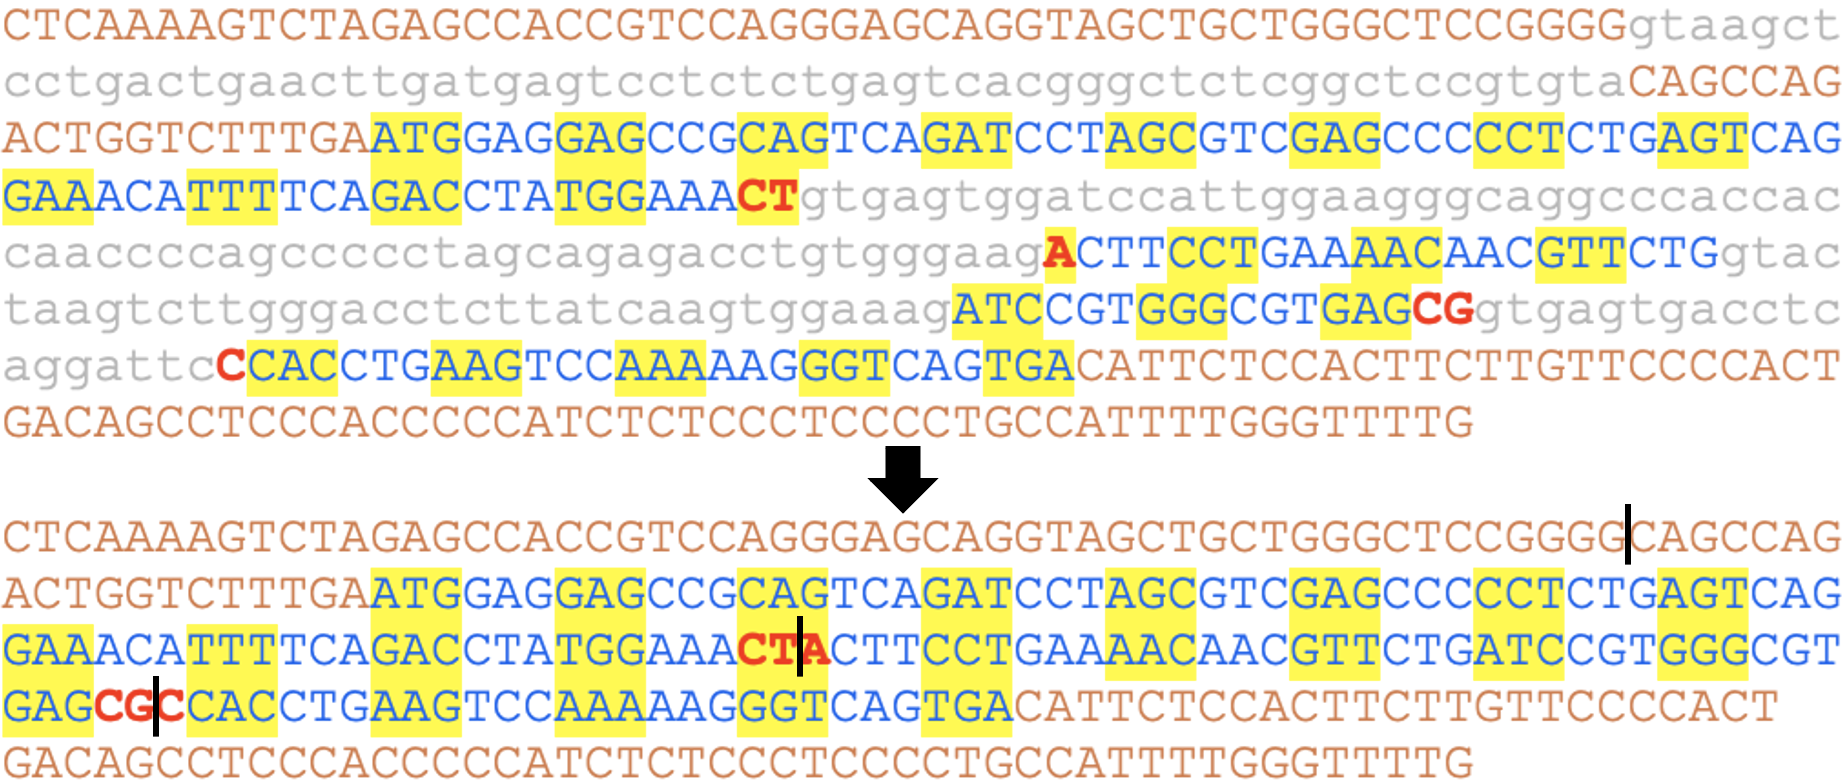
\includegraphics[width=0.48\textwidth]{images/gene.png}
  \caption{DNA Splicing Example}\label{fig:gene}
  \vspace{-3mm}
\end{figure}



In Figure \ref{fig:gene}, exons are in color, while introns are gray. The UTRs are orange, and the CDS is blue or red. Red nucleobases in the CDS indicate codons that are broken across splice sites. Notice how the 5' UTR is broken across the first two two exons, and the CDS spans the final four exons. Alternating highlights in the CDS are used for visibility of codons.  After excising the introns from the gene, the result is the contiguous sequence of exons at the bottom of Figure \ref{fig:gene}. The black vertical bars indicate splice sites. To perceptualize splicing, BioMus splits the chord for a spliced codon into half its original duration and places it at each end of the splice site: the chord will both close the exon that begins the codon and open the next exon that completes the codon. 

In this paper, we begin by examining relevant work in the field, and subsequently discuss the process of sourcing genetic data from the Ensembl database and its conversion to musical chords. Finally, examples of BioMus' sonification model are presented. 

\section{Related Work}

Sonofication of genetic material has been approached from a variety of angles. To specifically address accessibility of genomics to a wider audience, Takahashi and Miller converted genome-encoded protein sequences to piano notes in order to produce musical patterns that still adhere to the structure of the sequences. Like BioMus, Takahashi and Miller mapped codons in the CDS to chords. However, their scheme mapped pairs of amino acids to triads, with differing inversions distinguished individual amino acids within the pairs. The duration of each triad correlated to the frequency of its corresponding codon in the CDS. Unlike BioMus, Takahashi and Miller only consider the CDS, and do not consider how to represent spliced codons. %https://genomebiology.biomedcentral.com/articles/10.1186/gb-2007-8-5-405


Plaisier et al. also seek to increase accessibility to genomics by proposing a sonification model that is both entertaining and informative. They map each nucleotide to a specific note to bridge the gap between the monotonous appearance of traditional DNA sequence visualizations and the excitement expected in a display by a public audience. By using the Sonic Pi program for sonification, they crucially support real-time customization of the program, providing a link between DNA and live programming to further enhance public engagement. BioMus' sonification model perceptualizes a wider variety of bioligical structures than Plaisier et al.'s model %https://bmcresnotes.biomedcentral.com/articles/10.1186/s13104-0 w21-05685-7

In another sonification model, Ingalls et al. consider the sequence alignment problem, in which genetic sequences from the same gene but different species are compared to identify regions of similarity. Their tool \textsc{ComposAlign} translates genome-wide aligned data into a musical composition using a unique mapping of alignment information onto musical features. Their approach sonifies the presence and absence of nucleotides or amino acids in the alignment such that their assignment to the corresponding sequence (i.e. species) is clear. By mapping each character to a measure-long motif, rather than a single note or chord, \textsc{ComposAlign} achieves mapping rules that are modular and flexible. Sequence alignment is outside the scope of BioMus' current scheme, but may be an intriguing future direction. %https://dl.gi.de/bitstream/handle/20.500.12116/20313/93.pdf

\section{Converting DNA to Music}
\subsection{Obtaining Genetic Data}
BioMus's process of DNA sonification begins with the user specifying a desired species and gene. This information is passed to Ensembl's REST API to obtain Ensembl's choromomal coordinates of the gene's exons. These coordinates are sourced from the gene's \textit{canonical transcript}, the gene's transcript in Ensembl that is overall the most conserved and highly expressed, has the longest CDS, and is also represented in other major databases such as the NCBI \cite{ensembl_transcript_flags}. The exon coordinates also define the chromosomal coordinates of the intervening introns. Each pair of exon and intron coordinates is passed back to the Ensembl REST API to obtain the nucleobase sequences for each region, and the result is a list of alternating exons and introns. For instance, consider the abbreviated sequence obtained from Ensembl for the \textit{Homo sapiens} (human) TP53 tumor suppressor gene in Figure \ref{fig:pre_processed_seq_homo_sapiens_tp53}. Ellipses indicate omitted nucleobases for the sake of example.

\begin{figure}[h!]
\centering
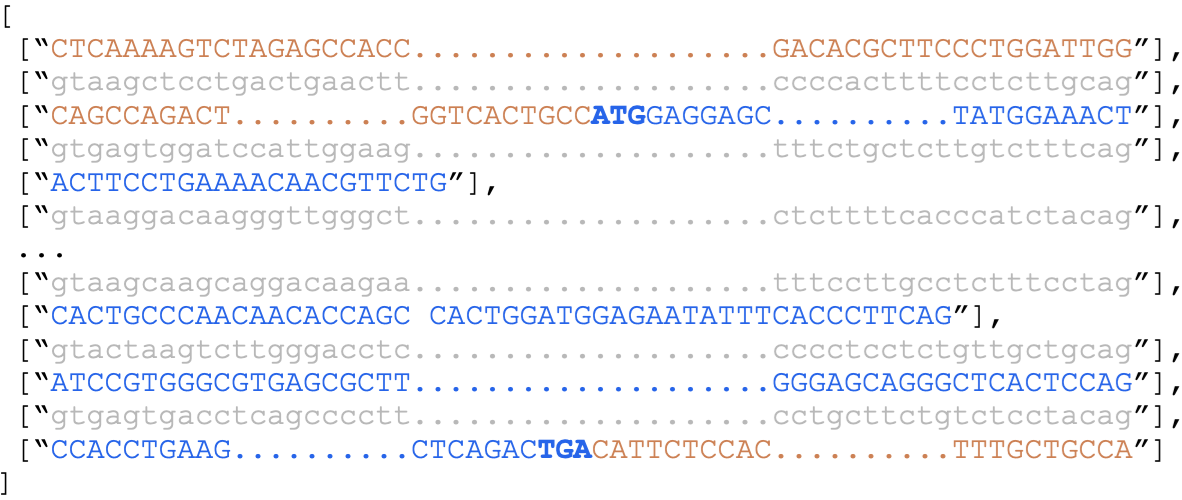
\includegraphics[width=0.48\textwidth]{images/pre_processed_seq_homo_sapiens_tp53_ABBREV}
  \caption{\textit{Homo sapiens}, TP53 Gene}\label{fig:pre_processed_seq_homo_sapiens_tp53}
  \vspace{-3mm}
\end{figure}

Exons are in color, while introns are in grey. Within the exons, the orange regions are the UTRs, and the blue regions are the CDS. Notice how the CDS begins with the bolded start codon ATG and ends with the bolded stop codon TGA. 

Now, the goal is to extract the 5' UTR from the list. In order to ensure the correct CDS, is necessary to verify the 5' UTR with Ensemble, since it may include multiple ATG start codons that do not signal the start of the CDS. This is not necessary for the 3' UTR, since once we know we are in the CDS, the first stop codon will always signal the end of the CDS and the beginning of the 3' UTR. We obtain the 5' UTR from Ensembl by querying the Ensembl REST API for the cDNA sequence of the canonical transcript. By requesting Ensembl to ``mask" the UTRs of the cDNA sequence by representing them in lowercase, we can successfully isolate the 5' UTR and extract it from the list in Figure \ref{fig:pre_processed_seq_homo_sapiens_tp53}. As seen in Figure \ref{fig:post_processed_seq_homo_sapiens_tp53}, we end up with a list of the 5' UTR regions (top), and a list of the CDS regions and introns (bottom).\cite{10.1162/artl_a_00325}

\begin{figure}[h!]
\centering
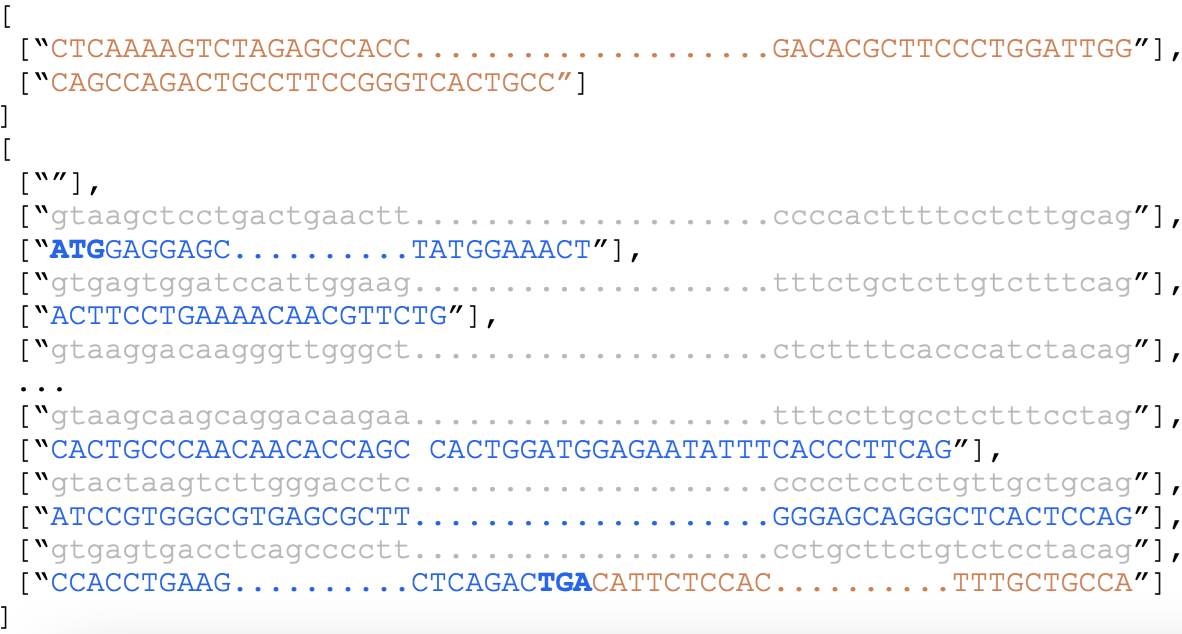
\includegraphics[width=0.48\textwidth]{images/post_processed_seq_homo_sapiens_tp53_ABBREV}
\vspace{-3mm}
  \caption{\textit{Homo sapiens}, TP53 Gene}\label{fig:post_processed_seq_homo_sapiens_tp53}
  \vspace{-3mm}
\end{figure}

We now have all the tools necessary to translate the genetic data into music.

\subsection{Conversion to MIDI}

MIDI conversion begins by using the MIDIUtil Python library to create a MIDI track with the tempo set to \musQuarter\;= 200 BPM. Subsequently, individual nucleobases in UTRs are mapped to minor dyads (two-note chords), codons in the CDS are mapped to major triads, and individual nucleobases in introns are mapped diminished triads. All chords are built within the octave C4-B4. This means that all chords built on the notes C through E will be in root position, and the remainder will be in inversion.

Sonification of the gene begins with the 5' UTR, and the initial key is set to C minor. No key changes occur in UTRs or introns; the key is exclusively changed in the CDS and is determined by the codon. Thus, before the CDS begins, all introns and the 5' UTR remain in the initial key of C minor. After the CDS begins, the key of an intron is determined by the final codon in the preceding exon (whether or not that codon is broken across the splice site). The stop codon terminating the CDS then determines the key of all subsequent introns as well as the 3' UTR.

To construct the dyads in the 5' and 3' UTRs, BioMus defines the following mapping of individual nucleobases to musical notes relative to the local musical key in Table  \ref{table:nucleobases}.

\begin{table}[h!]
\centering
\begin{tabular}{|l|l|}
\hline
A   & Tonic    \\ \hline
C, T & Mediant  \\ \hline
G   & Dominant \\ \hline
\end{tabular}
\caption{DNA Nucleobase Mappings}
\label{table:nucleobases}
\end{table}

The dyad corresponding to each nucleobase in a UTR is constructed with its base pair using the mapping in Table  \ref{table:nucleobases}. For instance, if the key is C minor and we encounter the nucleobase A or T, then the dyad will consist of the notes C (tonic) and E\musFlat \; (mediant). Together, the dyads outline a minor triad in the current key. Similarly, if we encounter the nucleobase C or G, then the dyad is E\musFlat \; and G (dominant). All UTR dyads are represented with quarter notes.

To construct the diminished triads in introns, BioMus again uses the mapping of individual nucleobases to musical notes in Table  \ref{table:nucleobases}. Initially, a dyad is constructed as in the UTRs (except with the dominant scale degree lowered a half step to form a diminished rather than a perfect fifth with the tonic). Then, we also add the diminished seventh scale degree from the local key to each dyad to construct the diminished triads. For instance, if the key is C minor and we encounter the nucleobase C or G, then the triad will consist of the notes C (tonic), E\musFlat \; (mediant), and B\musDoubleFlat\; (diminished seventh). Similarly, if we encounter the nucleobase A or T, then the triad will consist of the notes E\musFlat, G\musFlat \; (dominant), and B\musDoubleFlat. We use the term ``diminished triad" loosely here, since technically only the latter triad described fits the formal definition of a diminished triad, with two minor thirds stacked on top of one another. However, as both chords outline a diminished seventh chord, their sonority is similar enough that we dub them both diminished triads as a way of distinguishing them from major or minor chords. Like UTRs, all intron triads are represented with quarter notes. 

When the CDS begins, we map codons (groups of three nucleobases), rather than individual nucleobases, to chords. The first codon in the CDS is always ATG, the start codon, which is mapped to a C major triad and is given a half note duration, rather than a quarter note, as a signpost of the beginning of translation. Subsequent chords return to quarter notes. To further emphasize we are in a protein-coding region, the volume is doubled throughout the CDS. The volume is halved to its original value whenever we encounter an intron, and doubled again when we return to the CDS in the next exon. 

We also consider the scenario where the final codon of an exon in the CDS is broken across a splice site (i.e. the codon is split by the intervening intron). When an incomplete codon is encountered at the end of an exon in the CDS, the subsequent exon is referenced for the remainder of the codon. The spliced codon is then represented with an eighth note triad rather than a quarter note, and the same eighth note triad is played at the beginning of the next exon to indicate that the remainder of the codon is found there. This scenario is detailed in Figure \ref{fig:splice_site_example}, where exons are represented in color and introns are in gray. 

\begin{figure}[h!]
\centering
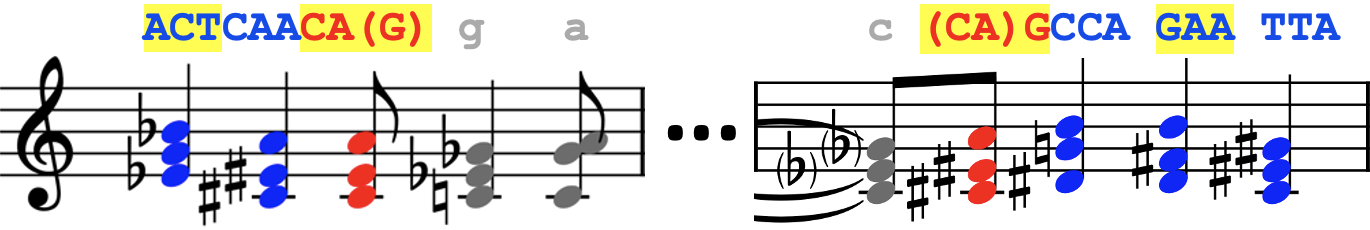
\includegraphics[width=0.38\textwidth]{images/splice_site_example}
  \caption{Spliced Codon Example}
  \label{fig:splice_site_example}
  \vspace{-3mm}
\end{figure}

The spliced codon CAG is in red, with the nucleobases CA in the first exon and G in the second. Notice how the same A augmented eighth note triad both closes the first exon and opens the second.

Thus far, we have demonstrated a novel means to conceptualize biological splicing by differentiating between UTRs, introns, and the CDSs, as well as emphasizing spliced codons. We now want to map codons in the CDS to chords in such a way that facilitaties the perception of biological translation. To do so,
we consider the amino acids the codons specify. To distinguish between amino acids, we seek an injective mapping between amino acids and musical keys. We do this by first solely considering the set of essential and nonessential amino acids (with which we can create a bijective mapping with the set of possible keys), and separately considering the set of conditionally essential amino acids (with which we can create an injective mapping with the set of possible keys).

Figures \ref{table:essential} and \ref{table:nonessential} explicate the chosen bijective mapping between the set of essential and nonessential amino acids and the set of possible keys. The codons that code for each amino acid are listed in the left hand column, and BioMus maps each to a major triad in the corresponding key in the right column. 

\vspace{-2mm}
\begin{table}[h!]
\centering
\begin{tabular}{|l|l|l|}
\hline
ATG & \begin{tabular}[c]{@{}l@{}}Methionine/\\Start Codon\end{tabular} & C                         \\ \hline
ATT, ATC, ATA & Isoleucine                        & C\musSharp \\ \hline
AAA, AAG &  Lysine                      & D                         \\ \hline
ACT, ACC, ACA, ACG & Threonine                       & E\musFlat  \\ \hline
TTT, TTC & Phenylalanine                       & E                         \\ \hline
TGG & Tryptophan             & F                         \\ \hline
\begin{tabular}[c]{@{}l@{}}TTA, TTG, CTT, CTC, \\CTA, CTG\end{tabular}  & Leucine                       & F\musSharp \\ \hline
CAT, CAC & Histidine                       & G                         \\ \hline
GTT, GTC, GTA, GTG &  Valine                      & A\musFlat  \\ \hline
\end{tabular}
\caption{Essential Amino Acids}
\label{table:essential}
\end{table}
\vspace{-5mm}
\begin{table}[h!]
\centering
\begin{tabular}{|l|l|l|}
\hline
AAT, AAC & Asparagine & A                        \\ \hline
GAT, GAC & Aspartate  & B\musFlat \\ \hline
GCT, GCC, GCA, GCG & Alanine    & B                        \\ \hline
\end{tabular}
\caption{Nonessential Amino Acids}
\label{table:nonessential}
\end{table}
\vspace{-2mm}

Next, we consider the set of nonessential amino acids. Tables \ref{table:essential} and \ref{table:nonessential} explicate the chosen injective mapping between this set and the set of possible keys. Notice that the mapping is also bijective between the nonessential amino acids and the set of natural keys. 

\begin{table}[h!]
\centering
\begin{tabular}{|l|l|l|}
\hline
TAT, TAC & Tyrosine                & C \\ \hline
TGT, TGC & Cysteine                & D \\ \hline
\begin{tabular}[c]{@{}l@{}}TCC, TCT, TCA, TCG, \\ AGT,  AGC\end{tabular}  & Serine                  & E \\ \hline
\begin{tabular}[c]{@{}l@{}}AGA, AGG, CGT, CGC, \\ CGA, CGG\end{tabular}  & Arginine                & F \\ \hline
CCT,  CCC, CCA, CCG & Proline                 & G \\ \hline
CAA, CAG, GAA, GAG  & \begin{tabular}[c]{@{}l@{}}Glutamine/\\Glutamic acid\end{tabular}  & A \\ \hline
GGT, GGC, GGA, GGG & Glycine                 & B \\ \hline
\end{tabular}
\caption{Conditionally Essential Amino Acids}
\label{table:conditionally_essential}
\vspace{-5mm}
\end{table}

This time, BioMus maps each codon to an augmented triad, rather than a major triad, in the corresponding key in the right column. 


Finally, we consider the stop codons, which do not code for amino acids and instead terminate the CDS. They are mapped to minor triads in the keys explicated in Table \ref{table:stop_codons}. 
\vspace{-2mm}
\begin{table}[h!]
\centering
\begin{tabular}{|l|l|}
\hline
UAA & C \\ \hline
UAG & E \\ \hline
UGA & G \\ \hline
\end{tabular}
\caption{Stop Codons}
\label{table:stop_codons}
\end{table}
\vspace{-3mm}

Each stop codon chord is given a half note duration and the volume is halved to signify the end of the protein-coding region. The subsequent minor dyads in the 3' UTR constituting the remainder of the gene return to quarter notes, and are in whatever key is dictated by the stop codon in Table \ref{table:stop_codons}. 



\section{Sample Music}

Figures \ref{fig:danio_rerio_start_translation} and \ref{fig:danio_rerio_end_translation} demonstrate the sonification of key sections in the TP53 tumor suppressor gene of the zebrafish \textit{Danio rerio}. The DNA sequence is shown above BioMus' sonification of each nucleobase or codon. Orange indicates a UTR, gray indicates an intron, and blue indicates the CDS. Red indicates CDS codons that are broken across splice sites. Alternating codons in the CDS are highlighted for visibility.

Figure \ref{fig:danio_rerio_start_translation} begins with the fragment of the 5' UTR concluding the gene's first exon. 

\begin{figure}[h!]
\centering
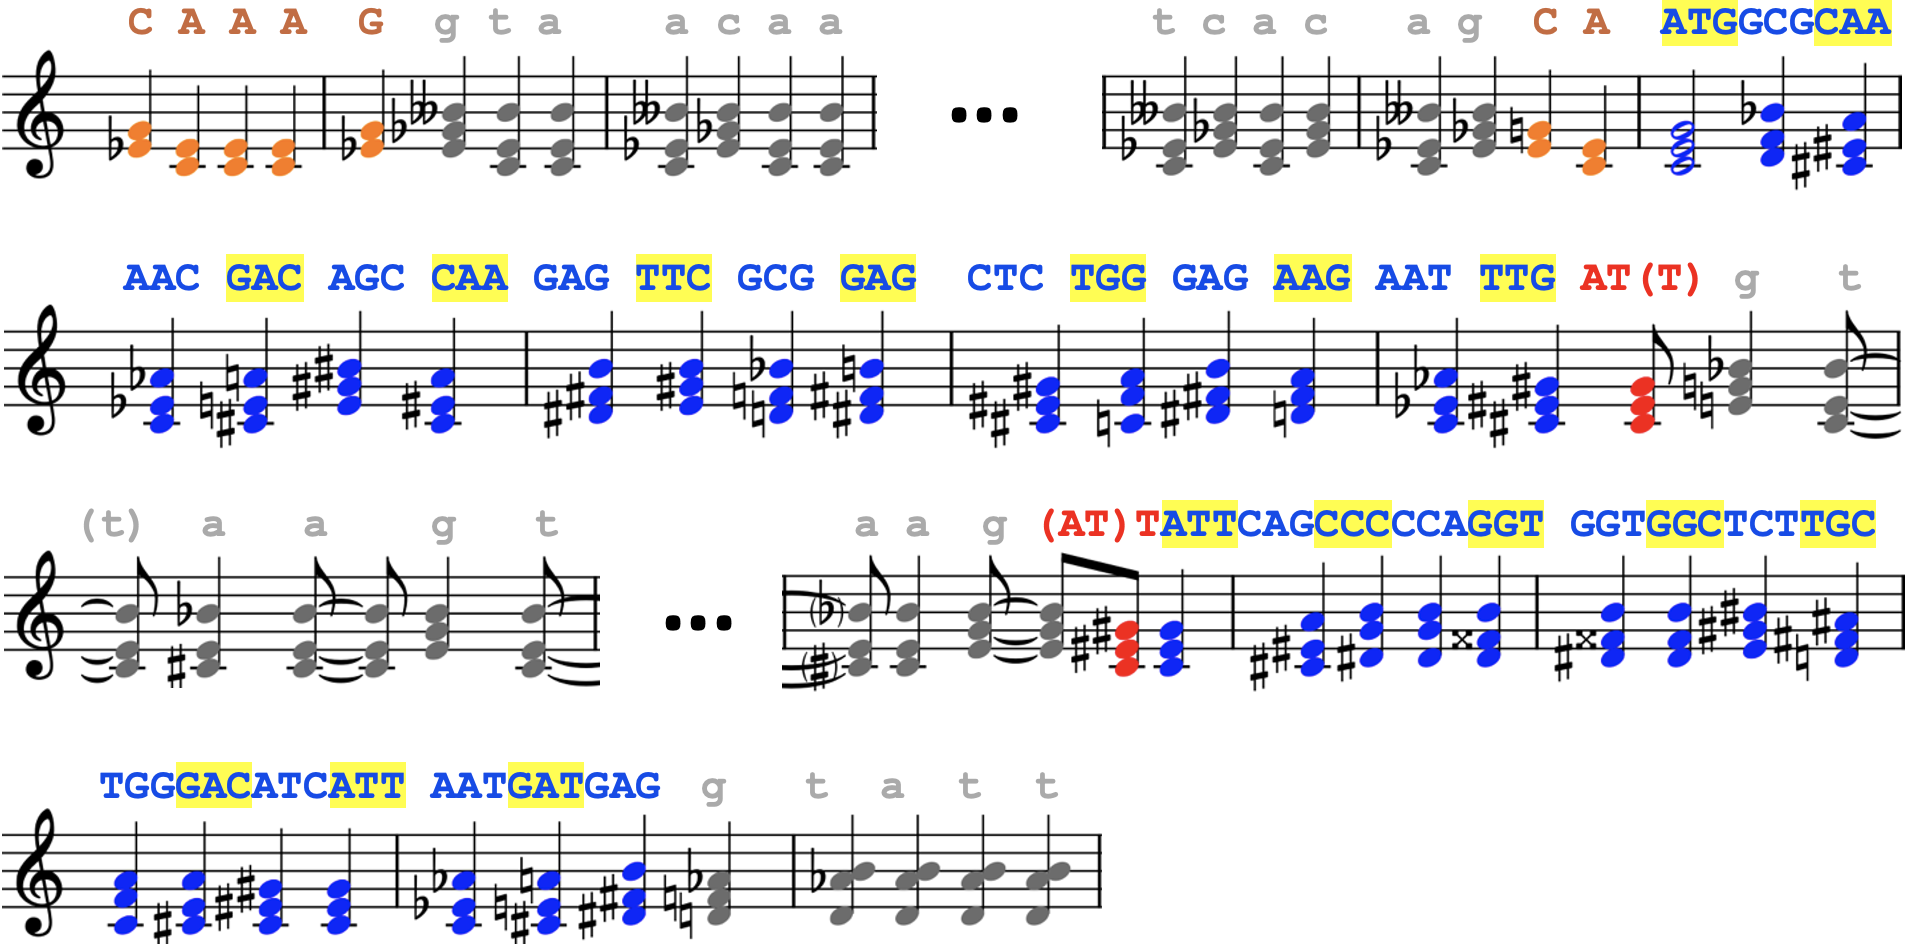
\includegraphics[width=0.48\textwidth]{images/danio_rerio_start_translation}
\vspace{-3mm}
  \caption{\textit{Danio rerio} TP53 Gene, Beginning of CDS}
  \label{fig:danio_rerio_start_translation}
  \vspace{-3mm}
\end{figure}

Notice how the opening key is C minor. The nucleobases A and T map to the dyad C-E\musFlat \; (tonic-mediant), and the nucleobases A and T map to the dyad C-E\musFlat \; (tonic-mediant). We then enter the gray region of the first intron, where diminished triads outline the C diminished seventh chord (notice how the perfect fifth G above the tonic becomes the diminished fifth G\musFlat, and each triad includes the addition of the diminished seventh B\musDoubleFlat). 

The second exon begins with the last two nucleobases of the 5'UTR, which again outlines the C minor triad, before beginning the CDS with the start codon ATG, which maps to a C major triad in in Table \ref{table:essential}. Notice how ATG maps to a half, rather than a quarter, note to signify the start of the protein-coding region.

From here, each CDS codon maps to a major or augmented triad based on tables \ref{table:essential} - \ref{table:conditionally_essential}. For instance, GCG codes for the nonessential amino acid alanine, which maps to a B major triad in Table \ref{table:nonessential}, while GAG codes for the conditionally essential amino acid glutamine, which maps to an A augmented triad in Table \ref{table:conditionally_essential}. 

Then, notice how the codon ATT, which codes for the essential amino acid isoleucine and maps to the C\musSharp\; major triad in red, is broken across the splice site between the second and third exons. The intervening intron assumes the key of the final codon of the previous exon and thus outlines a C\musSharp \; diminished seventh chord. 

Finally, notice how the third exon begins with the other ``half" (i.e.  remaining eighth note) of the C\musSharp\; major triad of the spliced ATT codon. This exon concludes with the complete codon GAG, which again codes for glutamine and maps to an A augmented triad in Table \ref{table:conditionally_essential}. The following intron assumes the same key of A, and outlines an A \; diminished seventh chord. Notably, if played, the volume in the CDS would be doubled relative to the rest of the sequence.

Figure \ref{fig:danio_rerio_end_translation} shows a fragment of the exon containing the end of the CDS. 

\begin{figure}[h!]
\centering
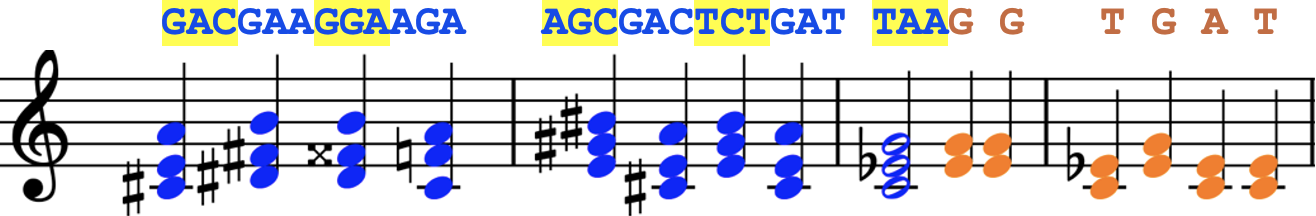
\includegraphics[width=0.48\textwidth]{images/danio_rerio_end_translation}
\vspace{-3mm}
  \caption{\textit{Danio rerio} TP53 Gene, End of CDS}
  \label{fig:danio_rerio_end_translation}
  \vspace{-3mm}
\end{figure}

The CDS terminates with the stop codon TAA, which maps to a C minor triad in Table \ref{table:stop_codons}. Notice how TAA maps to a half, rather than a quarter, note to signify the end of the protein-coding region. After this, we immediately enter the 3' UTR, which assumes the key of the stop codon and thus produces dyads outlining a C minor triad. 

\section{Conclusion}
BioMus serves as a bridge between bioinformatics, computer science, and music by giving both scientists and the general public a novel, creative means to aurally conceptualize the biological processes of DNA splicing and translation. The structure of the gene and its splice regions are illuminated by respectively mapping individual nucleotides in UTRs and introns to diminished chords and minor dyads, and breaking chords across splice sites just as their corresponding codons are. Translation is conveyed by mapping codons to major and augmented chords in the CDS based on the amino acids they code for. The chosen injective mapping between codons and musical keys also allows the listener to distinguish between essential, nonessential, and conditionally essential amino acids. BioMus' straightforward sonification model allows users to conceptualize the structure of DNA and the processes of splicing and translation whether or not they are career scientists, and opens to the door for visually impaired users to access these concepts without being constricted by traditional visual methods of genomic representation. 

In the future, BioMus would ideally sonify a greater variety and granularity of genomic structures. For instance, known mutations could be marked with dissonance. Furthermore, given a sample sequence and a target sequence, the similar regions of the sample sequence resulting from alignment with the target could be marked aurally by both new harmonies and rhythms. Finally, BioMus' current sonification scheme is intentionally linear to align with its vision of straightforward representation. Going forward, BioMus could benefit from modifying this scheme to integrate more complex rhythms and a larger sonic range, while still maintaining a clear musical distinction between genetic structures, in order to increase the musicality of its results.


\section{Acknowledgments}

I am very grateful to Professor Zachary Dodds of Harvey Mudd College for his mentorship throughout this project.


\bibliographystyle{iccc}
\bibliography{iccc}


\end{document}
